%
\documentclass[%
 reprint,
 amsmath,amssymb,
 aps,
]{revtex4-1}

\usepackage{graphicx}% Include figure files
\usepackage{dcolumn}% Align table columns on decimal point
\usepackage{bm}% bold math


\begin{document}


\title{ MODELO DIMENSIONAL VS MODELO TABULAR}
\author{Aquino Huallpa, Yaneth Virginia           }
\author{Damian Mamani, David Reynaldo 	  }
\author{Merino Quispe, Katerin Almendra 	  }
\author{Taquila Carazas Percy	  }
		
\affiliation{%
 Universidad Privada de Tacna \textbackslash Facultad de Ingenieria \textbackslash Escuela Profesional de Ingenieria de Sistemas
}%

\begin{abstract}
\begin{center}
\textbf{Resumen}
\end{center}

Se han investigado  en  areas,  de  incrementar  la  eficiencia  en  el almacenamiento y el acceso a las bases de datos analíticos, sobre cuyos resultados las grandes compañías han  introducido  productos  comerciales.  En  este  escenario,  Microsoft  SQL  Server ofrece  dos opciones  independientes para  la creación  de los  modelos analíticos,  el  modelo dimensional  y  el reciente modelo  tabular. El  presente articulo profundiza en las características y potencialidades de cada uno, proponiendo los criterios más importantes que, a juicio de los autores, se deben tener en cuenta al emprender  un  nuevo  proyecto.  
El  modelo  tabular  utiliza  técnicas  de  bases  de  datos  en  memoria  y almacenamiento  columnar,  con  algoritmos  de  compresión  avanzados,  lo  que  lo  convierte  en  una alternativa muy eficiente y atractiva en algunos contextos.  Se propone una solución computacional que brinda  a  los  especialistas  y  ejecutivos  tanto  visiones  particulares  como  integradoras  del  estado  del negocio,  aprovechándose  las  facilidades  recientes  que  proporciona  la  plataforma  de  Inteligencia  de Negocios  de  Microsoft  para  implementar  ambos  modelos, dimensional  y  tabular.
\begin{center}
\textbf{Abstract}
\end{center}
Research has been carried out in areas to increase efficiency in storage and access to analytical databases on the results of commercial data networks. In this scenario, Microsoft SQL Server offers two independent options for the creation of analytical models, the dimensional model and the recent tabular model. The present article deepens in the characteristics and potentialities of each one, proposing the most important criteria that, a judgment of the authors, must be taken into account when undertaking a new project.
The tabular model uses database techniques in memory and columnar storage, with advanced compression algorithms, which makes it a very efficient and attractive alternative in some contexts. It is proposed a computational solution that provides specialists and executives with both particular views and integrating the state of the business, taking advantage of the recent facilities provided by the Microsoft Business Intelligence platform to implement both dimensional and tabular models.
\end{abstract}
\maketitle
%\tableofcontents
\section {Introducción}\label{sec:1}
LOS AVANCES tecnológicos de los últimos años han
provocado una gran revolución, al incrementar la
disponibilidad de acceso a la información. A medida que ha
aumentado la cantidad de datos acumulados y las exigencias
de los directivos, han proliferado las necesidades de análisis
mucho más complejos para alcanzar el éxito. En este contexto
surge la Inteligencia de Negocios (BI, Business Intelligence)
que reúne un conjunto de metodologías, procesos,
arquitecturas y tecnologías que permiten transformar los datos
en información útil e importante para formular ideas
estratégicas, tácticas y operativas, eficaces para la toma de
decisiones . Numerosas compañías de software han
desarrollado plataformas que ofrecen a las empresas un
producto completo que responde a las diferentes etapas del
proceso de BI, a partir de las cuales es posible generar
soluciones de BI propias. La mayoría de los sistemas de
gestión de bases de datos que ofrecen herramientas para
realizar el procesamiento analítico de grandes volúmenes de
datos (OLAP, On Line Analytic Processing), se apoyan en la
tecnología de almacenamiento orientada a filas/registros (roworiented),
 optimizada para el procesamiento transaccional de los datos . 
Sin embargo, varios autores han defendido la
propuesta del almacenamiento lógico columnar, basado
esencialmente en la transposición de los ficheros para mejorar
el desempeño de las consultas. Mediante esta propuesta se
trata de beneficiar el procesamiento analítico de los datos,
caracterizado por demandas que requieren el agrupamiento o
la agregación de grandes cantidades de datos sobre unas pocas
columnas, desde la perspectiva de los índices de proyección a
través de las filas (column-oriented). 
%-----------------------------------------------------------------
\section{Objetivos}\label{sec:2}
\subsection{General:}
Comprender las bases de datos analíticas, y los diferentes modelos disponibles.
\subsection{Específicos:}
Aprender a desarrollar modelos tabulares, y las bases de su uso en informes.
Administrar y desplegar los modelos tabulares.

%-----------------------------------------------------------------
\section {Marco Teórico}

\subsection{MODELO DIMENSIONAL}

El modelado dimensional fue presentado a una amplia audiencia en la industria del almacén de datos por Ralph Kimball en 1997. Sin embargo, él no lo inventó. Los términos dimensiones y hechos, que son construcciones elementales en el modelado dimensional, se remontan a la década de 1960 cuando se realizó un proyecto de investigación conjunto entre la Universidad de Dartmouth y General Mills. El primer modelo dimensional fue presentado por AC Nielsen e IRI para describir los primeros marts de datos dimensionales para datos de ventas minoristas.\\
Un modelo dimensional es una técnica de estructura de datos optimizada para herramientas de almacenamiento de datos, está compuesto por tablas de "hechos" y "dimensiones".\\
Un modelo dimensional está diseñado para leer, resumir, analizar información numérica como valores, saldos, recuentos, pesos, etc. en un almacén de datos. \\

1. Elementos \\
- Hecho: son las medidas / métricas o hechos de su proceso comercial. Para un proceso comercial de ventas, una medición sería el número de ventas trimestral \\
- Dimensión: proporciona el contexto que rodea un evento de proceso de negocio, es una ventana para ver información en los hechos. \\
- Atributos: son las diversas características de la dimensión, se usan para buscar, filtrar o clasificar hechos. \\
- Tabla de hechos: es una tabla primaria en un modelo dimensional. \\
- Tabla de dimensiones: contiene dimensiones de un hecho, se unen a la tabla de hechos mediante una clave externa. \\

2. Pasos de modelado dimensional \\
- Identificar procesos de negocios \\
- Identificar grano (nivel de detalle) \\
- Identificar dimensiones \\
- Identificar hechos \\
- Construir esquema \\


%-------------------------------------------------
\subsection{VENTAJAS  DEL DIMENSIONAL}	

- Recuperación más rápida de datos
El modelado dimensional combina las tablas en el propio modelo, lo que permite a los usuarios recuperar datos más rápido al ejecutar consultas de unión en comparación con los otros enfoques. El esquema desnormalizado de un modelo dimensional está optimizado para ejecutar consultas ad hoc. Como resultado, complementa en gran medida los objetivos de inteligencia empresarial (BI) de una organización.

- Mejor comprensión de los procesos de negocio
La información en un modelo dimensional se almacena en tablas de hechos y dimensiones. Esta categorización de los datos en hechos y dimensiones, y la estructura entidad-relación de un modelo dimensional, presentan procesos de negocios complejos de una manera fácil de entender para los analistas.

- Flexible para cambiar
El marco de modelado dimensional hace que el diseño del almacén de datos sea extensible. El diseño se puede modificar fácilmente para incorporar nuevos requisitos comerciales o realizar ajustes. Se pueden agregar nuevas entidades en el modelo o se puede cambiar el diseño de las existentes para reflejar los procesos comerciales modificados.





%-------------------------------------------------

\subsection{MODELO TABULAR}
En términos muy simples un modelo tabular es una base de datos OLAP cuyo almacenamiento esta en memoria RAM. \cite{damian1}\\
Los modelos tabulares son bases de datos “en memoria” de Analysis Services. Gracias a los algoritmos de compresión avanzados y al procesador de consultas multiproceso, el motor analítico en memoria xVelocity (VertiPaq) ofrece un acceso rápido a los objetos y los datos de los modelos tabulares para aplicaciones cliente de reportes como Microsoft Excel y Microsoft Power View.\\
Los modelos tabulares admiten el acceso a los datos mediante dos modos: modo de almacenamiento en caché y modo DirectQuery. En el modo de almacenamiento en caché, puede integrar datos de varios orígenes como bases de datos relacionales, fuentes de distribución de datos y archivos de texto planos. \\
En el modo DirectQuery, puede omitir el modelo en memoria, lo que permite a las aplicaciones cliente consultar los datos directamente en el origen relacional (SQL Server).Analysis Services proporciona funciones de procesamiento analítico en línea (OLAP) y minería de datos para aplicaciones de Business Intelligence
Además su arquitectura permite que se generen modelos rápidamente ya que su implementación es sencilla y permite performance de rendimiento.\\
Los modelos tabulares están basados en columnas y no existe el concepto de agregaciones, lo que quiere decir, que cuando se realicen consultas sobre el mismo el motor de consulta solo trabajará con las columnas que figuren en la consulta.\\
Por último, en tabular no existe el concepto de “agregaciones” que existe en los cubos multidimensionales. El almacenamiento en los modelos tabulares está basado en columnas, esto es, que cuando se realiza una consulta MDX, el motor de consulta solo trabajará sobre las columnas especificadas en la consulta. \cite{damian2}
\begin{center}
	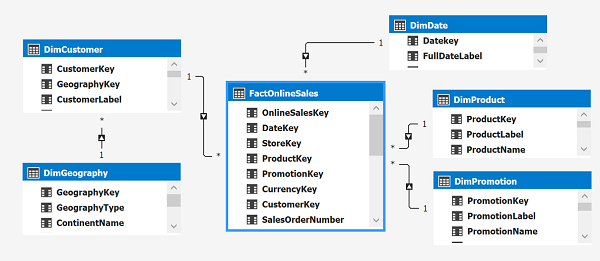
\includegraphics[width=9cm]{./Imagenes/modelotabular}
\end{center}
\newpage
%-------------------------------------------------
\subsection{VENTAJAS Y DESVENTAJAS DEL MODELO TABULARL}	
\subsubsection{Ventajas del Modelo Tabular} 
			\begin{itemize}
	 			
	 			\item Mucho más veloz en consultas.
	 			\item No requiere generar Aggregations (agregaciones) por lo que se simplifica el tiempo de procesamiento.
	 			\item Gracias al DAX (el lenguaje para acceder a los datos equivalente al MDX), tiene mayor flexibilidad para obtener información.
	 			\item Es intuitivo por lo que es mucho más rápido y fácil de entender e implementar.
	 			\item Se basa en modelos relacionales.
	 			
 			\end{itemize}
 		
\subsubsection{Desventajas del Modelo Tabular} 
			\begin{itemize}
				
				\item Las particiones no se procesaban en paralelo si no secuencialmente, lo que hace que sea más lento el procesamiento.
				\item No se pueden usar múltiples idiomas.
				\item Si son muchos datos tarda bastante en manejar configuraciones de diferentes particiones.
				\item El modelo tabular acapara demasiada memoria RAM y a su vez es dependiente de tal que afectará a otras aplicaciones
				
			\end{itemize} 	



%-------------------------------------------------

\subsection{SOLUCIÓN BI BASADA EN LOS MODELOS MULTIDIMENSIONAL Y TABULAR}	
Con el desarrollo del hardware, las tecnologías han
evolucionado ostensiblemente, favoreciendo el
aprovechamiento de las nuevas técnicas de gestión de bases de
datos en memoria (in-memory databases) y el almacenamiento
columnar para la optimización de las consultas en soluciones
analíticas.
 Un resultado de ello lo constituye Microsoft SQL
Server 2012 (y sus versiones posteriores), el cual ofrece dos
opciones independientes para la creación de los modelos
analíticos que representan la lógica del negocio, el clásico
modelo multidimensional y el reciente modelo tabular que no
constituye un remplazo del modelo multidimensional, sino
otra técnica para la instrumentación del procesamiento
analítico de los datos . 
El modelo tabular se ha convertido
en una alternativa interesante a considerar en el marco de la
toma de decisiones, especialmente en cuanto a la potenciación
de las funcionalidades de “autoservicio” .
El surgimiento de esta nueva y atractiva propuesta de
Microsoft para la concepción y desarrollo de soluciones
analíticas constituyó fuente importante de motivación para el
desarrollo de esta investigación, a través de la que se aportan
consideraciones en cuanto a:
 ¿Por qué se propone un nuevo modelo de análisis de datos cuando ya existía el modelo multidimensional con más de una década de explotación?;
¿Cuáles son las ventajas que ofrece el modelo tabular con
respecto a su precedente?; ¿En qué contextos se debe utilizar
uno u otro, o bien si ambos son necesarios? Las interrogantes
han sido analizadas en un entorno organizacional real,
específicamente en el Grupo Empresarial CIMEX.
El Grupo Empresarial CIMEX es líder nacional en el
mercado comercial mayorista y minorista, y tiene como
principal objetivo la adquisición y la comercialización de
productos y servicios. Adicionalmente constituye uno de los
principales referentes nacionales en cuanto al desarrollo de
herramientas de BI en función de mejorar los procesos de
dirección en la organización.
En el marco de la investigación se concibió y diseñó una
solución computacional basada en el paradigma de BI [1], a
través de la cual se implementaron los modelos
multidimensional y tabular sobre SQL Server 2012 Analysis
Services (SSAS). La solución desarrollada permitió realizar
análisis sobre los principales indicadores comerciales,
contables, económico-financieros y de recursos humanos de la
empresa y proporciona un ambiente para las consultas
dinámicas con funcionalidades de autoservicio, siguiendo una
de las más importantes tendencias de la industria en los
últimos años . Al mismo tiempo, constituyó un escenario
práctico real sobre el cual se exploraron los modelos
multidimensional y tabular en el procesamiento analítico de
los datos de la empresa, enriqueciendo las valoraciones
comparativas reportadas por otros autores . El
análisis de los modelos se llevó a cabo mediante cuatro
experimentos realizados sobre todas las sucursales de CIMEX,
obteniéndose como resultado un conjunto de consideraciones
generales en cuanto a las fortalezas y las debilidades de cada
enfoque.
Las contribuciones principales del trabajo son:
- Un análisis comparativo entre los modelos
multidimensional y tabular sobre el desarrollo de una
solución real de BI para una gran empresa.
- Concepciones generales sobre las fortalezas y las
debilidades de cada modelo para una elección más
objetiva ante diferentes escenarios.
El trabajo se organiza a continuación en cinco secciones.
En la sección II, se abordan los conceptos fundamentales del
paradigma de BI, haciendo énfasis en el procesamiento
analítico de los datos sobre la plataforma de Microsoft. En la
sección III, se expone la esencia del modelo tabular. En la
sección IV se enfatiza en el empleo de los modelos analíticos
multidimensional y tabular en la solución BI propia. En la
sección V se realiza una breve comparación de ambos
modelos sobre la base de resultados experimentales.
Finalmente se presentan las conclusiones y líneas futuras en la
sección VI. 

%-----------------------------------------------------------------
\subsection{COMPARACION ENTRE MODELO TABULAR Y MULTIDIMENSIONALS}	
completar
MODELO MULTIDIMENSIONALES:
Una base de datos multidimensional (MDB) es un tipo de base de datos que se ha optimizado para data warehouse y aplicaciones de procesamiento analitico en linea (OLAP).

\begin{center}
	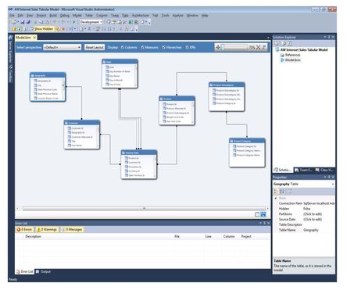
\includegraphics[width=9cm]{./Imagenes/1a}
\end{center}

MODELO TABULAR:
Las bases de datos Tabulares, son un nuevo tipo de base de datos que tienen la pecualiaridad de que trabajan siempre en memoria.

\begin{center}
	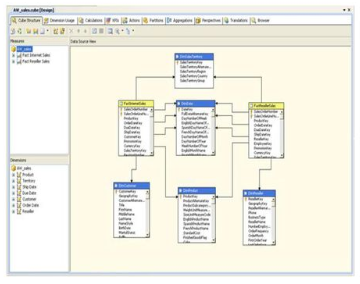
\includegraphics[width=9cm]{./Imagenes/1b}
\end{center}

COMPARACION ENTRE MODELO TABULAR Y MULTIDIMENSIONALES:

\begin{center}
	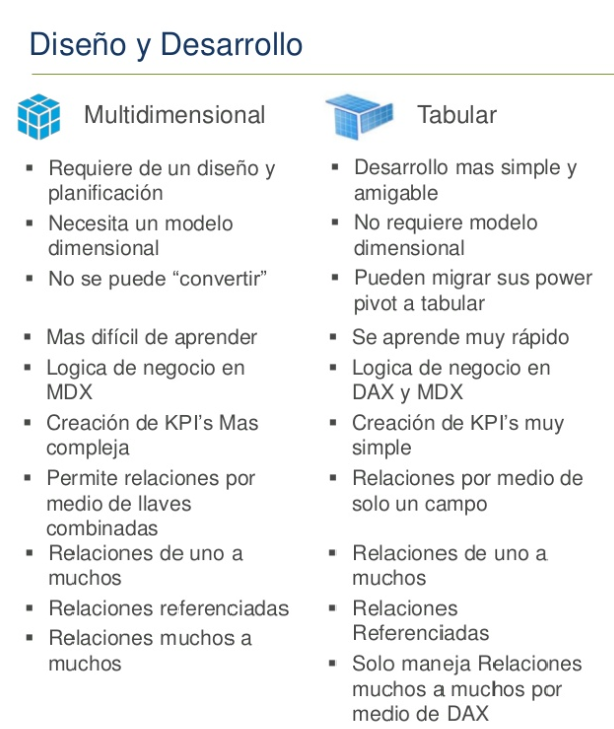
\includegraphics[width=9cm]{./Imagenes/1}
\end{center}
\begin{center}
	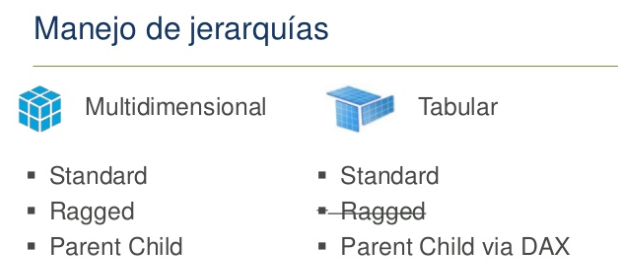
\includegraphics[width=9cm]{./Imagenes/2}
\end{center}
\begin{center}
	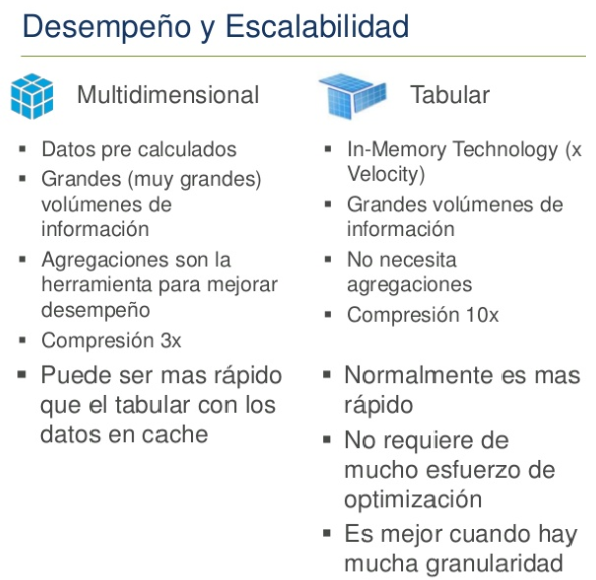
\includegraphics[width=9cm]{./Imagenes/3}
\end{center}
\begin{center}
	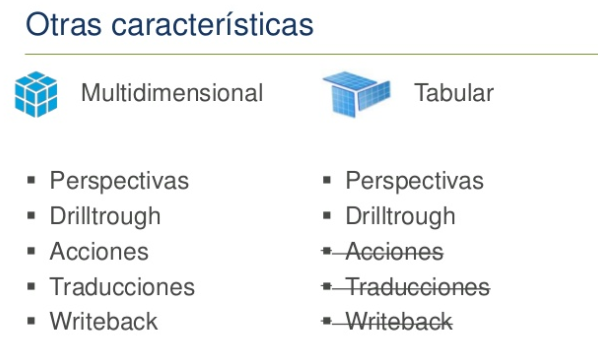
\includegraphics[width=9cm]{./Imagenes/4}
\end{center}
\begin{center}
	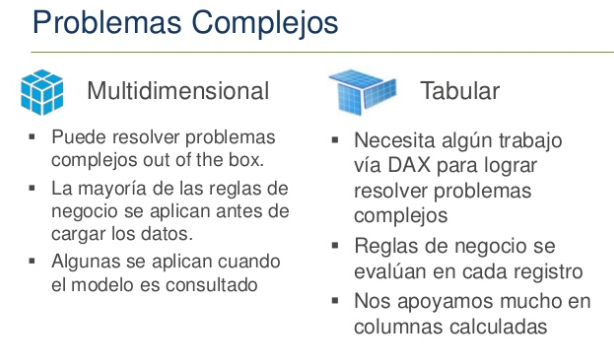
\includegraphics[width=9cm]{./Imagenes/5}
\end{center}
\begin{center}
	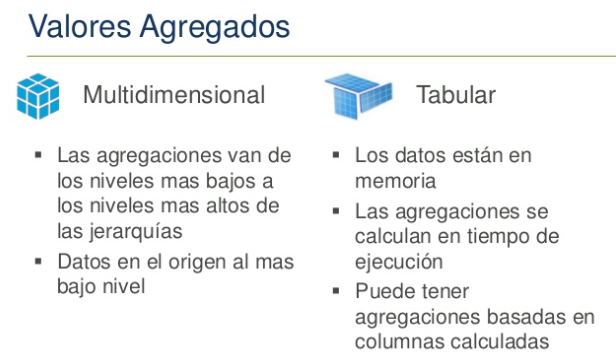
\includegraphics[width=9cm]{./Imagenes/6}
\end{center}
\begin{center}
	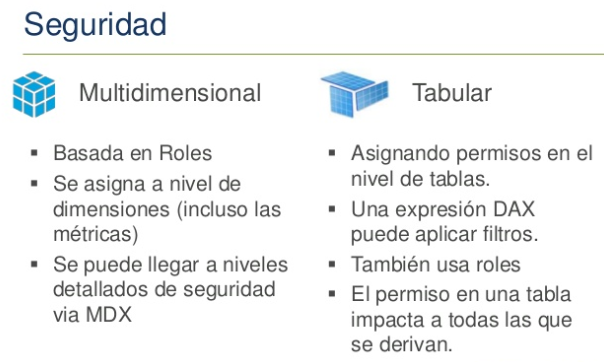
\includegraphics[width=9cm]{./Imagenes/7}
\end{center}

%-----------------------------------------------------------------
\section{Análisis}

\begin{itemize}
\item
En la realidad de las bases de datos, hay tres formas de mejorar el rendimiento: usar un mejor hardware, usar un mejor software y optimizar los datos. El modelado dimensional utiliza el tercer método. La justificación principal para el modelado dimensional es mejorar el rendimiento estructurando los datos para compensar la ineficiencia del procesamiento de unión. El propósito secundario es proporcionar una base consistente para el análisis. Hay momentos y lugares donde el modelado dimensional es apropiado y funcionará y otros tiempos y lugares donde es menos apropiado y realmente puede interferir con los objetivos de un almacén. 

\end{itemize}
%-----------------------------------------------------------------
\section{Conclusiones}

\begin{itemize}
\item 
En el modelo dimensional podemos usar dos modelos: estrella o copo de nieve. El estrella es el más sencillo además de ser quizás el más utilizado ya que su estructura es simple y hace que la extracción de datos sea más rápida, sin embargo para su uso mucha información debe estar contenida en cada una de las tablas de dimensión. Si se desea más orden en ese aspecto se puede utilizar el modelo copo de nieve sin embargo al existir más relaciones en el modelo este se volvería poco eficiente para buscar la información además de volverse complejo de mantener.

\end{itemize}


% Bibliografia.
%-----------------------------------------------------------------

\bibliographystyle{plain}
\bibliography{Bibliografia}
https://gravitar.biz/bi/sql-server-2012-multidimensional-vs-tabular/
https://slideplayer.es/slide/12390487/
\end{document}
